\documentclass[a4paper,10pt]{article}

\usepackage{graphicx}
\graphicspath{{sections/images/}}

\usepackage{amsmath}
\usepackage{amsfonts}
\usepackage{amssymb}
\usepackage{hyperref}
\usepackage[a4paper, top=2cm, bottom=2cm, left=2.5cm, right=2.5cm]{geometry}

\begin{document}
\begin{titlepage}
    \centering  
    \begin{figure}[ht]
        \centering
        
\includegraphics[width=\textwidth]{ise-logo.png}
    \end{figure}
    \vspace*{2cm} 
    
    {\Huge \textbf{Project Proposal:} \textit{Emotional Wellness Robot} \par}
    \vspace{4cm}
    
    {\large \textbf{Authors:} Tibet Buramarn, Kridbhume Chammanard, and Thitaya Divari \par}
    \vspace{1cm}
    {\large \textbf{Advisor:} Dr. Paulo Fernando Rocha Garcia and \par}
    {\large Ms. Kunpariya Siripanit \par}

    \vspace{3cm}
    
    {\large 2147416 Final Project I \par}
    {\large International School of Engineering (ISE) \par}
    {\large Chulalongkorn University \par}
    
    \vspace{2cm}
    
    {\large September 6, 2024 \par}
    
    \vspace*{\fill}
\end{titlepage}

\thispagestyle{empty}

\newpage
\begin{center}
        \item\section*{Abstract}
\end{center}
\large
Pookie, an AI-driven robot for promoting mental wellbeing, developed under advisory with Chula Student Wellness, aims to create an AI-driven companion to enhance mental well-being by promoting positivity. The robot aims to address “Terror Outbursts”, a future concern in Thailand involving an anxiety driven society, where the robot aims to alleviate feelings of stress and anxiety by providing a feeling of slowness and emotional attachment. The robot integrates computer vision, feature extraction, sensors, and actuators to address key customer needs in appearance, interactivity, and empathy. The general appearance features an anthropomorphic form with LED displays and sensors for interaction, drawing inspiration from existing robots like Kiki and Eilik, with future iterations expected to refine user experience and functionality based on feedback.  
\newpage
\begin{center}
        \item\section*{Acknowledgements}
\end{center}
The team expresses their sincere gratitude to Dr. Paulo Fernando Rocha Garcia, Ph.D., Assistant Professor of AI and Robotics at Chulalongkorn University, and Ms. Kunpariya Siripanit, Counseling Psychologist at Chula Student Wellness, Chulalongkorn University. Dr. Paulo’s expertise in artificial intelligence and robotics was instrumental in guiding the technical development of the emotional wellness robot, while Ms. Kunpariya’s insights into counseling psychology ensured the project’s alignment with mental health principles. The team also acknowledges the support provided by the faculty and staff of the International School of Engineering, whose assistance was invaluable throughout this project.
\normalsize

\newpage
\tableofcontents

\newpage
\begin{center}
\section{Topic Name}
\label{sec:topic}
\textbf{Project Title:} Your Project Title

\end{center}
\section{Research Background}
\label{sec:background}
This section should provide an overview of the research context, explaining the motivation behind the project and its significance. Include relevant statistics, historical background, and any industry-specific challenges that necessitate this research.

\newpage
\section{Objective}

\subsection{Main Objective Statement}
The primary objective of this project is to design, develop, and deploy an emotional wellness robot capable of recognizing and responding to stress and anxiety symptoms in users through the integration of AI technologies such as computer vision and natural language processing. The robot must fulfill all three key pillars of customer expectations in emotional wellness robots: design, interactivity, and empathy.

\subsection{Specific Goals}
\begin{itemize}
    \item Design an anthropomorphic robotic outer shell that resonates with the target customer segment.
    \item Design interactive verbal and non-verbal features for the robot, such as making sounds when the robot is touched on the head, with expert supervision from Chula Student Wellness (CUSW).
    \item Develop an accurate emotion detection algorithm that captures the user’s state of anxiety through speech emotion recognition and facial expression recognition.
    \item Develop empathetic human-robot interactions that promote emotional wellness within the customer.
    \item Finalize a customer-centric design obtained through market validation efforts.
    \item Conduct extensive testing and refinement based on user feedback.
\end{itemize}

\subsection{Measurable Outcomes}
\begin{itemize}
    \item Achieve a relative reduction in self-reported anxiety.
    \item Achieve a benchmark in accuracy metrics for emotion detection.
    \item Obtain an improved before-and-after positivity score.
\end{itemize}

\subsection{Relevance or Significance}
With “Terror Outbursts” being one of the major societal challenges in Thailand, there is a pressing need for accessible positivity promotion. Our robot aims to bridge the gap between traditional therapy sessions by providing immediate support to individuals struggling with anxiety.
\newpage
\section{Literature Survey and Review}
\label{sec:literature}
This section will review existing literature related to the project. Discuss previous studies, findings, and theories that are relevant to your research. Highlight gaps in the literature that your project aims to fill.

\newpage
\section{Project Concept Development}
\label{sec:concept}
Here, outline the conceptual framework of your project. Describe the methodology, tools, and technologies that will be used. Include diagrams or models if necessary to explain the concept.

\newpage
\section{Project Planning and Timeline}

The overall project will span a total of two academic semesters of the senior year (a total of approximately 8 months) and will comprise a set of goals for each semester. The project will be managed using an agile methodology, where by the end of the project, two deliverables will be obtained: MVP1 and MVP2. This section will break down the project planning and timeline for each MVP, as well as expected deliverables for each phase.

\subsection{Channels}

Throughout the project, two essential tools will be used to facilitate communication and task delegation within the project. The first tool is Discord, a multi-functional communication tool that is practical for meetings, scheduling events, and so on. Discord will be used as the primary communication tool for the members in the project, as well as for some advisors. The second tool is Jira, an agile project management tool that facilitates task delegation and software project management. Jira will be used to track the tasks of each member in the project, as well as to track software features and bugs within the project in the form of tickets for ease of audit. Additionally, it will also comprise the customer journey of each feature of the robot in the form of “user stories.”

\subsection{MVP 1 - Proof of Concept \& Customer-Centric Specifications}

MVP 1 will span the entirety of academic semester 1 (from September until December) and will focus on delivering a proof of concept of the project, as well as feature specifications that focus on the customers’ needs. MVP 1 will comprise three sprints, each lasting for around a month.

The project starts at MVP 1 Sprint 0, which focuses on preliminary research and feature definition. This sprint will span the entirety of September, and comprises the project proposal, in-depth customer journey, and technology specifications (such as specifically which AI models to be used). MVP 1 Sprint 0 will have two deliverables: the written project proposal and first progress report.

In the next phase, MVP 1 Sprint 1, which lasts from October to early November, we will focus on preliminary software development aimed towards providing a proof of concept for the emotion detection algorithm. For each AI model that will be used, we will allocate time for data collection, training, and iterative quality checks using real data. In general, emotion detection will comprise detection of facial expressions, Speech Emotion Recognition (SER), and Gesture Recognition technologies, utilizing computer vision and feature extraction technologies. In addition, there are plans to integrate context understanding into the robot using NLP technologies, but we will not include it in the scope. Additionally, the UX design will also be drafted, consisting of a complete customer journey for each feature, as well as a basic outer shell for the robot that fits the design specifications. Sprint 1 will have three deliverables: second progress report, third progress report, and completed prototypes for emotion detection.

In the last phase, MVP 1 Sprint 2, which lasts from November to early December, we will focus on acquiring the first batch of hardware components for the project and testing the emotion detection models on our selected microcontroller. The microcontroller must have enough compute power to perform inferences in real time. Additionally, Sprint 2 will involve market validation, which comprises testing on the customer segment to obtain feedback for improvement in the following semester. By the end of MVP 1, we expect a prototype that integrates software and hardware components on a feasible level.

\begin{figure}[ht]
    \centering
    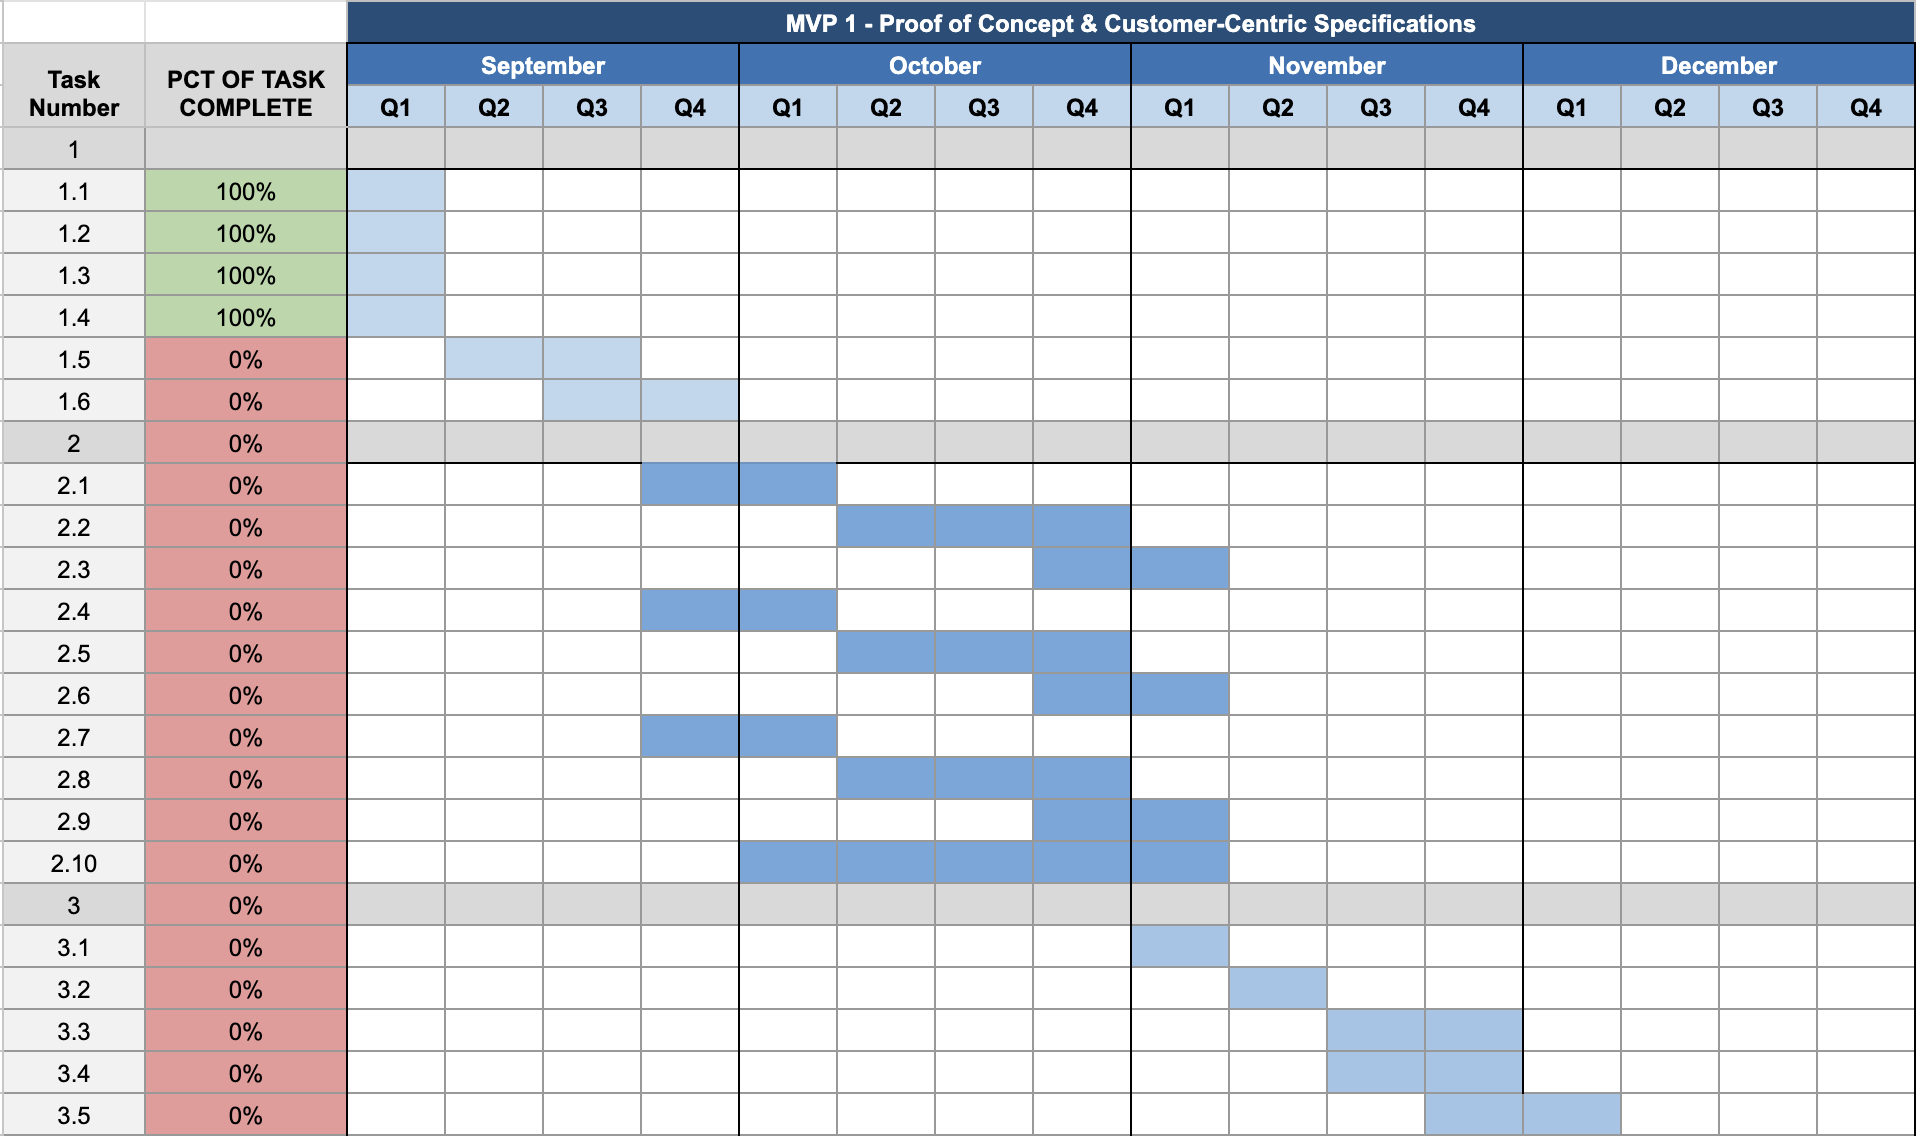
\includegraphics[width=\textwidth]{gantt-table.png}
    \caption{Gantt Chart for MVP 1 Timeline}
    \label{fig:gantt}
\end{figure}
\newpage
\subsection*{Task Number:}
\begin{enumerate}
\item\textbf{MVP 1 - Sprint 0}\\
1.1	Advisor Onboarding\\
1.2	Project Scoping\\
1.3	Project Scoping - Expert Interviews\\
1.4	Project Proposal\\
1.5	In-Depth Technology Specifications\\
1.6	E2E Customer Journey\\
\item\textbf{MVP 1 - Sprint 1}\\
2.1	Facial Expression Model - Data Collection\\
2.2	Facial Expression Model - Training/Testing\\
2.3	Facial Expression Model - Quality Testing\\
2.4	SER Model - Data Collection\\
2.5	SER Model - Training/Testing\\
2.6	SER Model - Quality Testing\\
2.7	Gesture Model - Data Collection\\
2.8	Gesture Model - Training/Testing\\
2.9	Gesture Model - Quality Testing\\
2.10 UX Design (Fusion360)\\
\item\textbf{MVP 1 - Sprint 2}\\
3.1	Parts Procurement\\
3.2	Jetson Orin/Nano Test\\
3.3	MVP 1 Integration \\
3.4	Market Validation\\
3.5	Final Presentation Preparations\\
\end{enumerate}

\newpage
\subsection{MVP 2 - Non-Commercial Prototype}

In this project proposal, the specific details of MVP 2 will not be disclosed. However, in general, MVP 2 will comprise three sprints, similar to MVP 1, but will focus on integration of the emotion detection algorithm with hardware components to create an output. MVP 2 will last the entirety of academic semester 2, and is expected to deliver a fully functional prototype, but will not be implemented to the extent of commercialization. Additionally, MVP 2 will focus on user testing, involving measurable metrics mentioned in the objectives section. The prototype will not encompass full consideration of security, safety, and real usage, but will focus on fulfilling the customer demands of appearance, interactivity, and empathy.

\subsection{Resource Allocation}

The project team comprises three senior engineering students. The roles for the project will be designated as follows: project manager, project engineer for product development, and project engineer for software development. The project manager is responsible for overseeing the entire project, delegating tasks, managing the timeline, and creating engagements with advisors from ISE and Chula Student Wellness. They are expected to streamline work processes for the project engineers and professionally check deliverables before submission. The project engineers are separated into two categories: product development and software development. The product development engineer will be responsible for UX design through CAD software, gathering hardware components, and managing the budget for doing so. The software development engineer will be responsible for overseeing all software initiatives, as well as managing DevOps practices within the project.

\subsection{Budget Allocation}

While the exact hardware components for the robot cannot be deduced yet, the table below will illustrate an approximate allocation of the budget provided for the project. Note that the budget specified is the maximum that was allocated for expenditure. The budget for each component may vary, but should never exceed the maximum allocated budget.

\begin{table}[ht]
\centering
\begin{tabular}{|l|l|}
\hline
\textbf{Component} & \textbf{Maximum Allocated Budget (THB)} \\ \hline
Microcontroller & 30,000 \\ \hline
Camera & 5,000 \\ \hline
Microphone & 5,000 \\ \hline
Electronics & 15,000 \\ \hline
Chassis and Framework & 5,000 \\ \hline
Decorative Components & 5,000 \\ \hline
LED Display & 5,000 \\ \hline
Miscellaneous & 5,000 \\ \hline
\textbf{Maximum Expenditure} & \textbf{75,000} \\ \hline
\end{tabular}
\caption{Approximate Budget Allocation for Hardware Components}
\end{table}

\newpage
\section{Theory and Technical Backup}

\subsection{Hardware Features}

The physical design of the robot is anthropomorphic-centric, with elements of animals as well. The robot will be around 12 inches tall, comprising various integrated hardware components. Starting from the top, the robot’s head will consist of a 3D printed sphere, and eyes made from an integrated LED display, which will be used as a form of interaction with the user. In addition, the head will also house the camera and microphone, used to receive image and sound inputs for processing within the microcontroller. Next, the robot’s body will consist of a large chassis to house the electrical components and the microcontroller. The body will also consist of motors located on the arms to allow for minor arm movement. Lastly, touch sensors will be placed in certain parts of the robot to imitate petting interaction. This design is akin to many desktop companion robots for promoting mental wellness, such as Kiki or Eilik, with the core difference being in the integration of various emotion detection methods.

\subsection{Software Features - Overview}

The robot comprises two main features: emotion detection and interaction. Emotion detection is an initiative to incorporate empathy for the customer experience with the robot, using computer vision to analyze facial expressions, as well as speech emotion recognition to analyze tone and pitch. Given predicted emotional status, the robot will be programmed to provide interaction in two forms: verbal and non-verbal. Verbal interactions consist of noises made by the robot, whereas non-verbal interactions comprise physical actions from the robot such as arm movement or changes in the LED display resembling its eyes.

\subsection{Emotion Detection Model - Facial Expression Recognition}

Facial expression recognition is a core technique in emotion detection systems, crucial for understanding non-verbal emotional cues in humans. Recent advancements have centered on using Convolutional Neural Networks (CNNs) to detect and classify facial emotions with high accuracy. OpenFace \cite{baltrusaitis2018} and VGGFace \cite{zhang2023} are among the most prominent models in this field. These models extract key facial features—such as eye movement, mouth shape, and eyebrow positions—from images and videos to classify emotions like happiness, anger, and sadness. CNNs have demonstrated strong performance by learning spatial hierarchies of features, allowing them to detect subtle changes in facial expressions, even in complex or dynamic environments. Such models are pivotal in creating emotionally responsive robots, as they allow real-time emotion tracking through visual input.

\subsection{Emotion Detection Model - Speech Recognition}

Speech recognition for emotional detection focuses on analyzing vocal characteristics to infer emotional states. Key prosodic features such as pitch, tone, and rhythm are crucial indicators of emotions in speech. Recent methods have employed Recurrent Neural Networks (RNNs) and Long Short-Term Memory (LSTM) networks for processing audio data, while newer approaches utilize transformer models like BERT \cite{devlin2019}. These models capture the temporal dependencies in spoken language, enabling the system to interpret emotions more accurately. LSTMs are particularly effective at maintaining contextual information over time, which is vital for understanding emotions that are expressed through vocal modulations. The integration of these techniques allows robots to engage in emotionally intelligent conversations by understanding the user's mood through their voice.
\newpage
\subsection{Testing}

The testing of the robot will comprise both internal and external components. In terms of internal components: The emotion detection model should achieve a benchmark score in accuracy metrics, or a similar number on a different scale. Since both the computer vision and speech emotion recognition (SER) datasets will be discretely labeled, quantitative measurement of accuracy will be feasible. For instance, the speech recognition model may classify a person’s voice as either normal or anxious.

On the other hand, in terms of external components, user testing will involve supervision and validation from Chula Student Wellness. Questionnaires will be developed to obtain the required information accordingly, representative questions include:

\begin{itemize}
    \item \textbf{Self-Report on Anxiety}
    \begin{enumerate}
        \item Before using Pookie, how would you rate your anxiety levels from 1-10? Please provide your rating now and when you’re at your most anxious.
        \item After using Pookie, how would you rate your anxiety levels from 1-10? Please provide your rating now and when you’re at your most anxious.
    \end{enumerate}
    \item \textbf{Positivity Promotion}
    \begin{enumerate}
        \item Before using Pookie, how would you rate your general positive feelings in life from 1-10?
        \item After using Pookie, how would you rate your general positive feelings in life from 1-10?
    \end{enumerate}
    \item \textbf{Attachment}
    \begin{enumerate}
        \item After using Pookie for 1 week, do you feel more attached to it?feelings in life from 1-10?
    \end{enumerate}
\end{itemize}

While these are examples of questions that will be asked, proper guidance from Chula Student Wellness will be given as well during the testing stage.
\newpage
\section{Project Outcome}
\label{sec:outcome}
This section should describe the expected outcomes of the project. What deliverables will be produced? How will the results be measured and evaluated?

\newpage
\section{Summary and Real Benefit to Industry}

\subsection{Summary}
In summary, the project focuses on developing an emotional wellbeing robot that promotes mental wellness and positivity for users under the influence of stress and anxiety. The robot will utilize technologies such as computer vision and natural language processing to recognize and respond to emotional cues in real time, providing consistent and empathetic support. With a focus on design, interactivity, and empathy, the robot is tailored to meet the needs of Gen Z and younger millennials in promoting mental wellbeing. The project is structured around two academic semesters, employing an agile methodology to deliver two key prototypes, MVP1 (Proof of Concept) and MVP2 (A Fully Functional Design).
The development process is guided by insights from Dr. Paulo Fernando Rocha Garcia, Ph.D., Assistant Professor of AI and Robotics at Chulalongkorn University, and Ms. Kunpariya Siripanit, a counseling psychologist at Chulalongkorn University, ensuring that the robot not only meets technical standards but also aligns with mental health principles. This project offers a scalable, innovative solution that addresses the increasing prevalence of anxiety disorders, positioning the robot as a sustainable alternative to traditional mental health support methods.

\subsection{Benefits}

\textbf{Direct Impact on the Industry:}  
This project will significantly benefit the mental health field, specifically targeting patients with general anxiety and stress, which comprises a massive customer segment. In particular, mental wellbeing robots are an important initiative in countering “Terror Outbursts” in Thailand. By leveraging AI to detect and respond to emotions through facial expressions and voice analysis, these robots can reduce reliance on human intervention in mental positivity promotion. Additionally, the project will enhance service quality by offering consistent promotion of mental well-being, effectively addressing unmet mental health needs.

\textbf{Scalability and Long-Term Value:}  
With recent studies indicating a 55\% increase in anxiety disorders globally from 1990 to 2019, affecting approximately 301 million people worldwide \cite{javaid2023}, these robots will become increasingly essential. Their ability to offer real-time, personalized assistance will not only improve individual well-being but also contribute to the long-term sustainability of mental health care systems. While the project will remain in the proof of concept and prototyping stage, it aims to provide an innovative approach to mental wellbeing, potentially scaling to commercial use in the future.
\newpage
\section{Workload or Responsibilities}
\label{sec:workload}
Outline the distribution of workload among the project team members. Specify the responsibilities assigned to each team member and their expected contribution to the project.


\newpage
\addcontentsline{toc}{section}{References}
\bibliographystyle{IEEEtran}
\bibliography{sections/references}

\end{document}
